% Run with: `pdflatex -shell-escape docs/tikz/flowchart.tex`;
% Depends on the external `pdf2svg` tool, here using its path in LLR machines

\documentclass[crop,tikz,convert={outext=.svg,command=\unexpanded{/opt/exp_soft/llr/pdf2svg/bin/pdf2svg \infile\space\outfile}},multi=false]{standalone}
\usepackage{amsmath}
\usetikzlibrary{shapes.geometric, calc, shapes.multipart, arrows.meta, positioning,
  backgrounds, bending}
% Tikz pictures
\newlength{\unit} \setlength{\unit}{.4cm}

\newcommand{\twolines}[2]{
  \begin{tabular}{c}
    \textbf{#1} \\ \textbf{#2}
  \end{tabular}
}


\newlength{\hdist} \setlength{\hdist}{6.\unit}
\newlength{\vdist} \setlength{\vdist}{3.\unit}
\newlength{\minhdist} \setlength{\minhdist}{3.\hdist}
\newlength{\minvdist} \setlength{\minvdist}{3.\vdist}
\newcommand{\mylinewidth}{0.15\unit}

\tikzset{
  % Diamonds
  mydiam/.style={diamond, draw=black, thick,
    minimum width=0.2\minhdist, minimum height=0.2\minvdist, fill=yellow!100},
  % Red box
  myredbox1/.style={rectangle, draw=black, fill=purple!50, rounded corners,
    minimum width=\minhdist, minimum height=\minvdist},
  % Blue box big
  mybluebox1/.style={rectangle, draw=black, fill=blue!50,
    minimum width=\minhdist, minimum height=\minvdist},
  % Blue box small
  mybluebox2/.style={rectangle, draw=black, fill=blue!50,
    minimum width=0.5\minhdist, minimum height=0.6\minvdist},
  % Green box
  mygreenbox1/.style={rectangle, draw=black, fill=green!40, rounded corners,
    minimum width=\minhdist, minimum height=0.5\minvdist},
  % Pale green box
  mypalegreenbox1/.style={rectangle, draw=black, fill=green!10, rounded corners,
    inner sep=2pt, dashed, minimum width=\minhdist, minimum height=0.5\minvdist},
  % Dashed box 1
  mydashbox1/.style={rectangle, draw=black, fill=gray!10, inner sep=3pt, dotted,
    minimum width=4.6\minhdist, minimum height=1.7\minvdist},
  % Dashed box 2
  mydashbox2/.style={rectangle, draw=black, fill=gray!10, inner sep=3pt, dotted,
    minimum width=1.2\minhdist, minimum height=3.5\minvdist},
  % Arrows
  myarrow/.style={line width=\mylinewidth,->,>=stealth},
  myarrowdashed/.style={line width=\mylinewidth,->,>=stealth, dashed},
  myarrow2/.style={line width=\mylinewidth,->,stealth-stealth},
  myarrowbend/.style={line width=\mylinewidth,-{>[flex=0.9]},>=stealth},
  bigarrow/.style={line width=1.5cm, arrows={-Triangle Cap[line width=1cm]}, draw=gray!75},
  condarrow/.style={line width=.05cm, arrows={-Stealth[]}, draw=black}
}  

\begin{document}

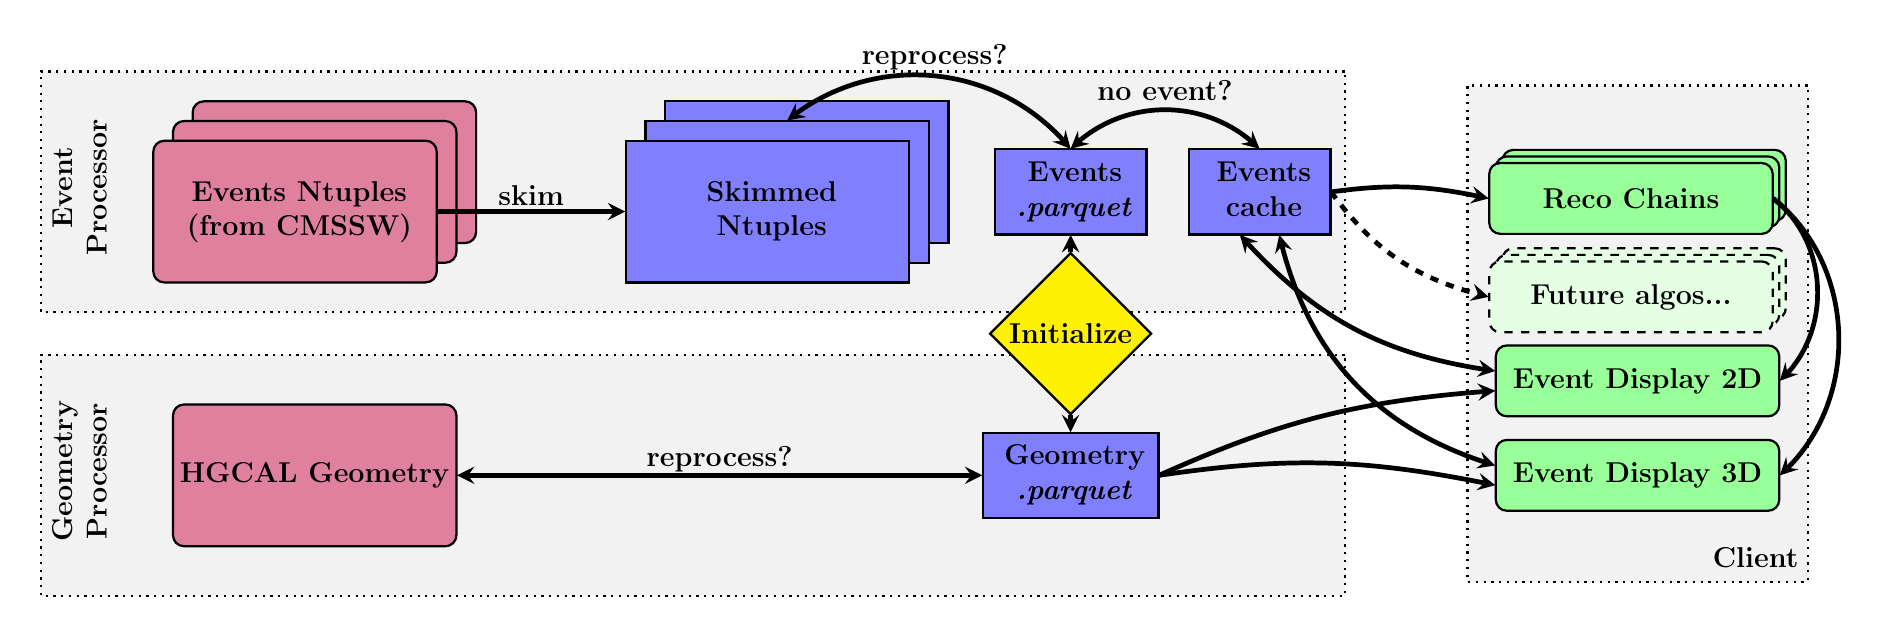
\begin{tikzpicture}[node distance=2cm, thick, scale=.5, every node/.style={transform shape},
  background rectangle/.style={fill=white}, show background rectangle]

  %%%%%%%%%%%%%%%%%%%%%%%%%%% 
  %%%%%% TOPOLOGY %%%%%%%%%%%
  %%%%%%%%%%%%%%%%%%%%%%%%%%% 

  \newcommand{\nrows}{7}
  \newcommand{\ncols}{15}
  \newcommand{\nrowsmid}{4}

  \newlength{\width} \setlength{\width}{\ncols\hdist}
  \newlength{\height} \setlength{\height}{\nrows\vdist}

  \newcommand{\mybend}{45}
  
  %%%%%%%%%%%%%%%%%%%%%%%%%%%%%%%%%%%%%%%%%%%% 
  %%%%%% ABSOLUTE POSITION COORDINATES %%%%%%%
  %%%%%%%%%%%%%%%%%%%%%%%%%%%%%%%%%%%%%%%%%%%% 

  \coordinate (top_left)     at (0,\height);
  \coordinate (top_right)    at (\width,\height);
  \coordinate (bottom_left)  at (0,0);
  \coordinate (bottom_right) at (\width,0);

  \coordinate (mid) at (\width/2,\height/2);
  \coordinate (mid_left) at (0,\height/2);
  \coordinate (mid_right) at (\width,\height/2);

  %%%%%%%%%%%%%%%%%%%%%%%%%%%%%%%%%%%%%%%%%%%% 
  %%%%%% RELATIVE POSITION COORDINATES %%%%%%%
  %%%%%%%%%%%%%%%%%%%%%%%%%%%%%%%%%%%%%%%%%%%% 

  \foreach \i in {1,...,\nrows}{
    \foreach \j in {1,...,\ncols}{
      \coordinate(COORD\i_\j) at (\j*\hdist, \i*\vdist);
    }
  }

  % Each object has its own coordinate
  \coordinate (entuple_c)  at (COORD\nrows_1);
  \coordinate (skim_c)     at (COORD\nrows_6);
  \coordinate (eparquet_c) at (COORD\nrows_9);
  \coordinate (ecache_c)   at (COORD\nrows_11);
  \coordinate (chains_c)   at (COORD\nrows_\ncols);
  \coordinate (future_c)   at ($ (chains_c) - (0,2.5) $);
  
  \coordinate (gntuple_c)    at (COORD1_1);
  \coordinate (gparquet_c)   at (COORD1_9);
  \coordinate (gdisplay2d_c) at (COORD3_\ncols);
  \coordinate (gdisplay3d_c) at (COORD1_\ncols);

  \coordinate (init_c) at (COORD\nrowsmid_9);

  \coordinate (gproc_c) at ($ (COORD1_5) - (0,0) $);
  \coordinate (eproc_c) at ($ (COORD\nrows_5) + (0,0.) $);
  \coordinate (client_c) at (COORD4_\ncols);
  
  %%%%%%%%%%%%%%%%%%%%%%%%%%% 
  %%%%%% NODES %%%%%%%%%%%%%%
  %%%%%%%%%%%%%%%%%%%%%%%%%%% 

  % Geometry processor
  \node (gproc) [mydashbox1] at (gproc_c) {};
  \node[rotate=90, thick] at ($ (gproc) - (15.5,0) $) {\huge \twolines{Geometry}{Processor}};

  % Event processor
  \node (eproc) [mydashbox1] at (eproc_c) {};
  \node[rotate=90, thick] at ($ (eproc) - (15.5,0) $) {\huge \twolines{Event}{Processor}};
  
  % Client
  \node (client) [mydashbox2] at (client_c) {};
  \node[align=left, thick] at ($ (client) - (-3.0,5.7) $) {\huge \textbf{Client}};

  % Event ntuples
  \foreach \i in {1,...,-1}{
    \ifnum\i=-1
    \node (entuple\i) [myredbox1] at ($ (entuple_c) + (\i/2,\i/2) $)
    {\huge \twolines{Events Ntuples}{(from CMSSW)}};
    \else
    \node (entuple\i) [myredbox1] at ($ (entuple_c) + (\i/2,\i/2) $)
    {};
    \fi
  }

  % Skimmed ntuples
  \foreach \i in {1,...,-1}{
    \ifnum\i=-1
    \node (eskim\i) [mybluebox1] at ($ (skim_c) + (\i/2,\i/2) $)
    {\huge \twolines{Skimmed}{Ntuples}};
    \else
    \node (eskim\i) [mybluebox1] at ($ (skim_c) + (\i/2,\i/2) $)
    {};
    \fi
  }

  % Events parquet
  \node (eparquet) [mybluebox2] at (eparquet_c) {\huge \twolines{Events}{\textit{.parquet}}};

  % Events cache
  \node (ecache) [mybluebox2] at (ecache_c) {\huge \twolines{Events}{cache}};

  % Geometry
  \node (gntuple) [myredbox1] at (gntuple_c) {\huge \textbf{HGCAL Geometry}};

  % Geometry parquet
  \node (gparquet) [mybluebox2] at (gparquet_c) {\huge \twolines{Geometry}{\textit{.parquet}}};

  % Initialization
  \node (init) [mydiam] at (init_c) {\huge \textbf{Initialize}};

  % Event display 2D
  \node (gdisplay2d) [mygreenbox1] at (gdisplay2d_c) {\huge \textbf{Event Display 2D}};

  % Event display 3D
  \node (gdisplay3d) [mygreenbox1] at (gdisplay3d_c) {\huge \textbf{Event Display 3D}};

  % Reco Chains
  \foreach \i in {1,...,-1}{
    \ifnum\i=-1
      \node (chains) [mygreenbox1] at ($ (chains_c) + (\i/6,\i/6) $)
      {\huge \textbf{Reco Chains}};
    \else
      \node (future) [mygreenbox1] at ($ (chains_c) + (\i/6,\i/6) $)
      {};
    \fi
  }
  
  % Future...
  \foreach \i in {1,...,-1}{
    \ifnum\i=-1
    \node (future) [mypalegreenbox1] at ($ (future_c) + (\i/6.,\i/6.) $)
    {\huge \textbf{Future algos...}};
    \else
    \node (future) [mypalegreenbox1] at ($ (future_c) + (\i/6,\i/6) $)
    {};
    \fi
  }

  % Tiny blocks inside RecHits GPU
  % \node (rh_gpu_1) [rechitsIn, below of=rh_gpu, yshift=\shiftTinyBlocksY, xshift=-1.65cm, scale=\scaleLettersTiny]
  % { CE-E 
  
  %%%%%%%%%%%%%%%%%%%%%%%%%%% 
  %%%%%% RELATIVE POS %%%%%%%
  %%%%%%%%%%%%%%%%%%%%%%%%%%% 

  \coordinate (relpos1) at ([yshift=\unit] top_left.south);
  \coordinate (relpos2) at ([yshift=\unit] top_right.south);
  
  %%%%%%%%%%%%%%%%%%%%%%%%%%% 
  %%%%%% ARROWS %%%%%%%%%%%%%
  %%%%%%%%%%%%%%%%%%%%%%%%%%% 
  
  %%%% \draw [arrow] (top_right) -- (top_left);
  %%%% \draw [arrow] (rh_fromSoA) -- (relpos1) -| ([xshift=-1.8cm] clue_cpu.north);

  % Event arrows
  \draw [myarrow] (entuple-1.east) to node[black,yshift=\unit]{\huge \textbf{skim}} (eskim-1.west);
  \draw [myarrow2] (eskim0.north) to [bend left=\mybend]
  node[black,yshift=1.2\unit]{\huge \textbf{reprocess?}}  (eparquet.north);
  \draw [myarrow2] (eparquet.north) to[bend left=\mybend]
  node[black,yshift=1.2\unit]{\huge \textbf{no event?}} (ecache.north);
  \draw [myarrow] (ecache.east) to [bend left=10] (chains.west);
  \draw [myarrowdashed] (ecache.east) to [bend left=-20] (future.west);
  \draw [myarrow2] ($ (ecache.south) - (.5,0) $) to [bend left=-20] ($ (gdisplay2d.west) + (0,.25) $);
  \draw [myarrow2] ($ (ecache.south) + (.5,0) $) to [bend left=-30] ($ (gdisplay3d.west) + (0,.25) $);
  
  % Geometry arrows
  \draw [myarrow2] (gntuple.east) to node[black,yshift=\unit]{\huge \textbf{reprocess?}} (gparquet.west);
  \draw [myarrow] (gparquet.east) to [bend left=10] ($ (gdisplay2d.west) - (0,.25) $);
  \draw [myarrow] (gparquet.east) to [bend left=10] ($ (gdisplay3d.west) - (0,.25) $);

  % Init arrows
  \draw [myarrow] (init.north) -- (eparquet.south);
  \draw [myarrow] (init.south) -- (gparquet.north);
  % \draw [myarrowbend] ($ (init.west) + (.5,.5) $) arc (30:330:1cm);

  % Reconstruction chain arrows
  \draw [myarrow] (chains.east) to [bend left=50] (gdisplay2d.east);
  \draw [myarrow] (chains.east) to [bend left=50] (gdisplay3d.east);  

  \foreach \i in {1,...,\nrows}{
    \foreach \j in {1,...,\ncols}{
      \fill[red] (COORD\i_\j) circle (0.001);
    }
  }
  
\end{tikzpicture}

\end{document}
